\documentclass[12pt,spanish,a5paper,landscape]{article}
\usepackage[utf8]{inputenc}
\usepackage{babel}
\usepackage{listings}
\usepackage{mathpazo}
\usepackage{courier}
\usepackage{textcomp}
\usepackage[parfill]{parskip}
\usepackage{xcolor}
\usepackage{tikz}
\usepackage{geometry}
\usepackage{enumitem}
\usepackage{microtype}

\newcommand{\onelinerule}{\rule[2.3ex]{0pt}{0pt}}
\newcommand{\twolinerule}{\rule[6.2ex]{0pt}{0pt}}
\newcommand{\respuesta}{\framebox[\textwidth]{\twolinerule}}
\newcommand{\nombre}{%
  \begin{tikzpicture}[xscale=.4,yscale=.7]
    \draw (0, 0) rectangle (22, 1);
  \end{tikzpicture}%
}
%\newcommand{\rol}   {\framebox[0.3\textwidth]{\onelinerule}}
\newcommand{\rol}{%
  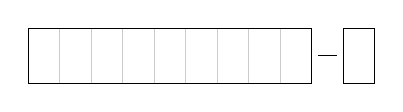
\begin{tikzpicture}[xscale=.4,yscale=.7]
    \draw[gray!40] ( 0, 0) grid      ( 9, 1);
    \draw          ( 0, 0) rectangle ( 9, 1);
    \draw          (10, 0) rectangle (11, 1);
    \draw (9 + .2, .5) -- (10 - .2, .5);
  \end{tikzpicture}%
}
\newcommand{\li}{\lstinline}
\providecommand{\pond}[1]{[{\small\textbf{#1\%}}]}

\lstdefinelanguage{py}{%
  classoffset=0,%
    morekeywords={%
      False,class,finally,is,return,None,continue,for,lambda,try,%
      True,def,from,nonlocal,while,and,del,global,not,with,print,%
      as,elif,if,or,yield,assert,else,import,pass,break,except,in,raise},%
    keywordstyle=\color{black!80}\bfseries,%
  classoffset=1,
    morekeywords={int,float,str,abs,len,raw_input,exit,range,min,max,%
      set,dict,tuple,list,bool,complex,round,sum,all,any,zip,map,filter,%
      sorted,reversed,dir,file,frozenset,open,%
      array,zeros,ones,arange,linspace,eye,diag,dot},
    keywordstyle=\color{black!50}\bfseries,%
  classoffset=0,%
  sensitive=true,%
  morecomment=[l]\#,%
  morestring=[b]',%
  morestring=[b]",%
  stringstyle=\em,%
}

\lstdefinelanguage{testcase}{%
  moredelim=[is][\bfseries]{`}{`},%
  backgroundcolor=\color{gray!20},%
}

\lstdefinelanguage{file}{%
  frame=single,%
}

\lstset{language=py}
\lstset{basicstyle=\ttfamily}
\lstset{columns=fixed}
\lstset{upquote=true}
\lstset{showstringspaces=false}
\lstset{rangeprefix=\#\ }
\lstset{includerangemarker=false}

\newlist{certamen}{enumerate}{1}
\setlist[certamen]{%
  label=\arabic*.,
  font=\LARGE\bfseries,%
  labelindent=-.5in,%
  leftmargin=0pt,%
  labelsep=1em%
}


\lstset{language=py}
\setlist[enumerate]{leftmargin=0pt}

\begin{document}
  \pagestyle{empty}
  \thispagestyle{empty}

  \part*{Control 4, lunes 1--2}
  \newpage

  El carioca es un juego de naipes típico de Chile.
  Cada jugador recibe una mano de varias cartas,
  numeradas del 1 al 13.

  Cuando un jugador tiene tres cartas con el mismo número,
  se dice que tiene un trío.

  \begin{enumerate}
    \item
      Escriba la función \li!contar_valores(cartas)!,
      que reciba como parámetro una lista de cartas,
      y retorne un diccionario que asocie a cada carta
      la cantidad de veces que aparece.
      \lstinputlisting[
        linerange=CASO\ 1-FIN\ CASO\ 1,
      ]{lunes-1-2.py}

    \item
      Escriba la función \li!tiene_trio(cartas)!
      que retorne un valor booleano
      indicando si la lista \li!cartas! tiene o no un trío.
      \lstinputlisting[
        linerange=CASO\ 2-FIN\ CASO\ 2,
      ]{lunes-1-2.py}

  \end{enumerate}
  \newpage

  \part*{Control 4, lunes 3--4}
  \newpage

  Los precios de los productos de un supermercado
  están almacenados en un diccionario como el siguente:
  \lstinputlisting[
    linerange=EJEMPLO\ PRECIOS-FIN\ EJEMPLO\ PRECIOS,
  ]{lunes-3-4.py}

  \begin{enumerate}
    \item
      Escriba la función \li!producto_mas_caro(precios)!,
      que reciba como parámetro el diccionario de precios,
      y retorne el nombre del producto más caro.
      Si hay más de un producto más caro,
      retorne cualquiera de ellos.
      \lstinputlisting[
        linerange=CASO\ 1-FIN\ CASO\ 1,
      ]{lunes-3-4.py}

    \item
      Una compra puede ser representada como un diccionario
      en que se asocia a cada producto
      la cantidad de unidades que se comprará.

      Escriba la función \li!monto_total(precios, compra)!,
      que reciba como parámetros el diccionario de precios
      y el diccionario de la compra,
      y retorne el monto total a pagar por la compra.
      \lstinputlisting[
        linerange=CASO\ 2-FIN\ CASO\ 2,
      ]{lunes-3-4.py}

  \end{enumerate}
  \newpage

  \part*{Control 4, martes 1--2}
  \newpage

  Una escuelita mantiene el registro de notas de los niños
  en un diccionario como el siguiente:
  \lstinputlisting[
    linerange=EJEMPLO\ NOTAS-FIN\ EJEMPLO\ NOTAS,
  ]{martes-1-2.py}

  \begin{enumerate}

    \item
      Escriba la función \li!calcular_promedios(notas)!
      que reciba como parámetro el diccionario de notas,
      y retorne un diccionario que asocie a cada niño su promedio.
      \lstinputlisting[
        linerange=CASO\ 1-FIN\ CASO\ 1,
      ]{martes-1-2.py}

    \item
      Escriba la función \li!clasificar_ninos(notas)!
      que reciba como parámetro el diccionario de notas
      y retorne un diccionario cuyas únicas dos llaves sean
      \li!'Aprobados'! y \li!'Reprobados'!.
      Los valores del diccionario deben ser, respectivamente,
      las cantidades de niños aprobados y reprobados.
      \lstinputlisting[
        linerange=CASO\ 2-FIN\ CASO\ 2,
      ]{martes-1-2.py}

  \end{enumerate}

  \newpage

  \part*{Control 4, martes 3--4}
  \newpage

  Se hizo una encuesta en varias ciudades.
  La encuesta consistía en una única pregunta,
  cuyas posibles respuestas eran \li!A!, \li!B! y \li!C!.
  Las respuestas de los encuestados de cada ciudad
  están almacenadas en un diccionario como el siguiente:
  \lstinputlisting[
    linerange=EJEMPLO\ RESPUESTAS-FIN\ EJEMPLO\ RESPUESTAS,
  ]{martes-3-4.py}

  \begin{enumerate}

    \item
      Escriba la función \li!resultados_encuesta(respuestas)!
      que reciba como parámetro el diccionario de respuestas,
      y retorne un diccionario asociando a cada respuesta
      el total de encuestados que la contestó:
      \lstinputlisting[
        linerange=CASO\ 1-FIN\ CASO\ 1,
      ]{martes-3-4.py}

    \item
      Escriba la función \li!porcentaje_respuesta_ciudad(respuestas, r, c)!,
      que reciba como parámetros el dicconario de respuestas,
      una respuesta \li!r! y una ciudad \li!c!.
      La función debe retornar el porcentaje de encuestados que respondió
      la respuesta \li!r! en la ciudad \li!c!.
      \lstinputlisting[
        linerange=CASO\ 2-FIN\ CASO\ 2,
      ]{martes-3-4.py}


  \end{enumerate}

\end{document}

